
\chapter{Additional Plots and Results}\label{appendix:result}

\begin{figure}[!h]
  \centering
  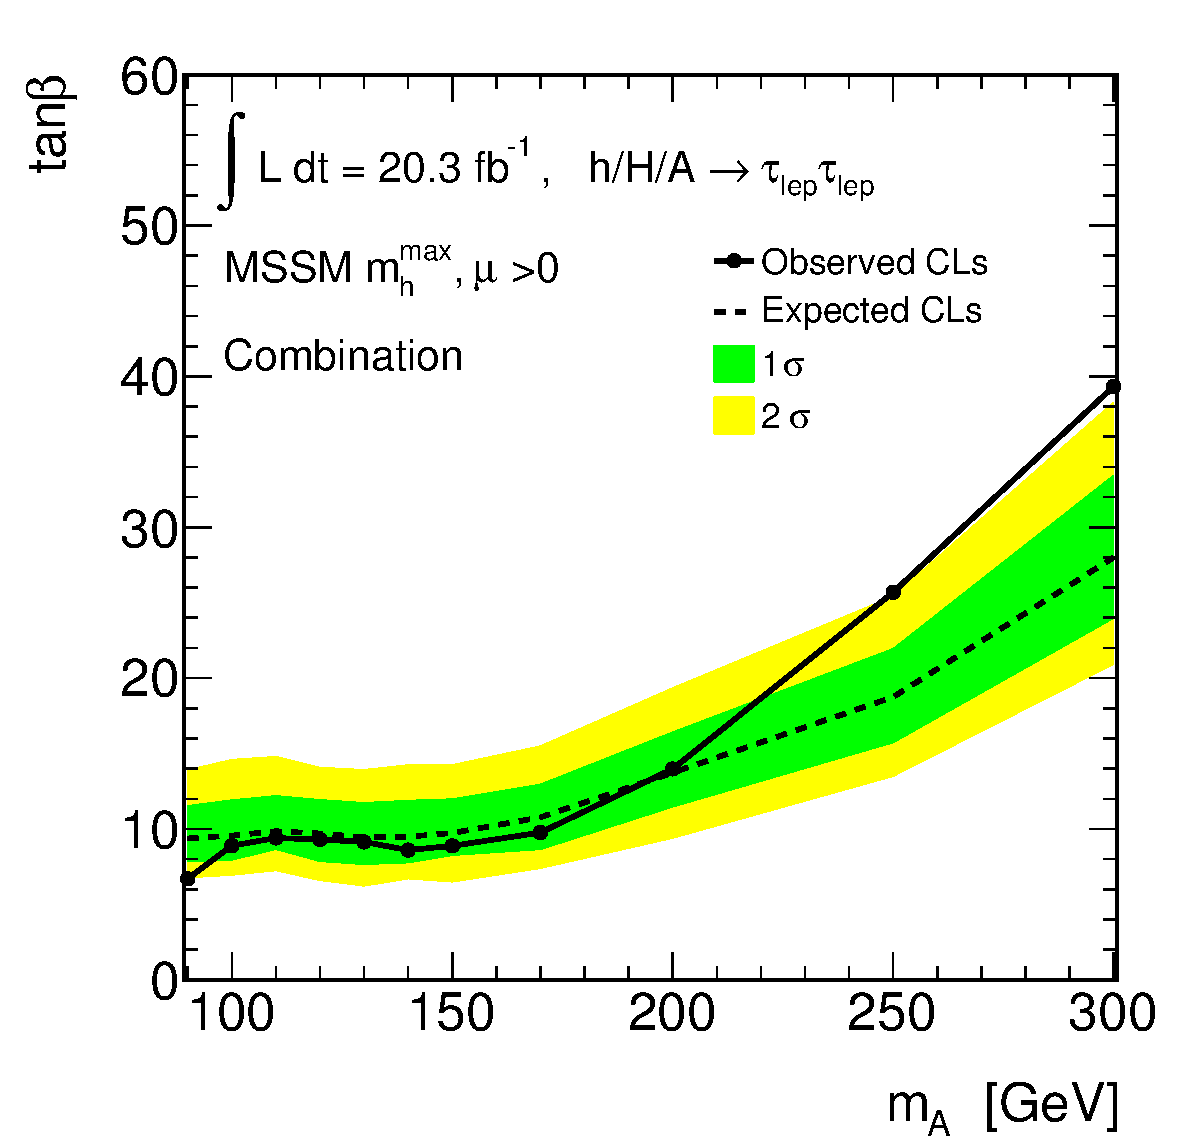
\includegraphics[width=0.7\textwidth]{figure/limits/comb_reg_spin.pdf}
  \caption{Expected and observed  exclusion limits at the $95\%$ $CL_s$ confidence-level for MSSM Higgs bosons production 
   interpreted in the  $m_A - \tan\beta$ parameter space of the $m_h^{max}$ scenario. 
	Combined result of the  b-tagged and b-vetoed category is shown.}
\end{figure}

\begin{figure}[tp]
  \centering
  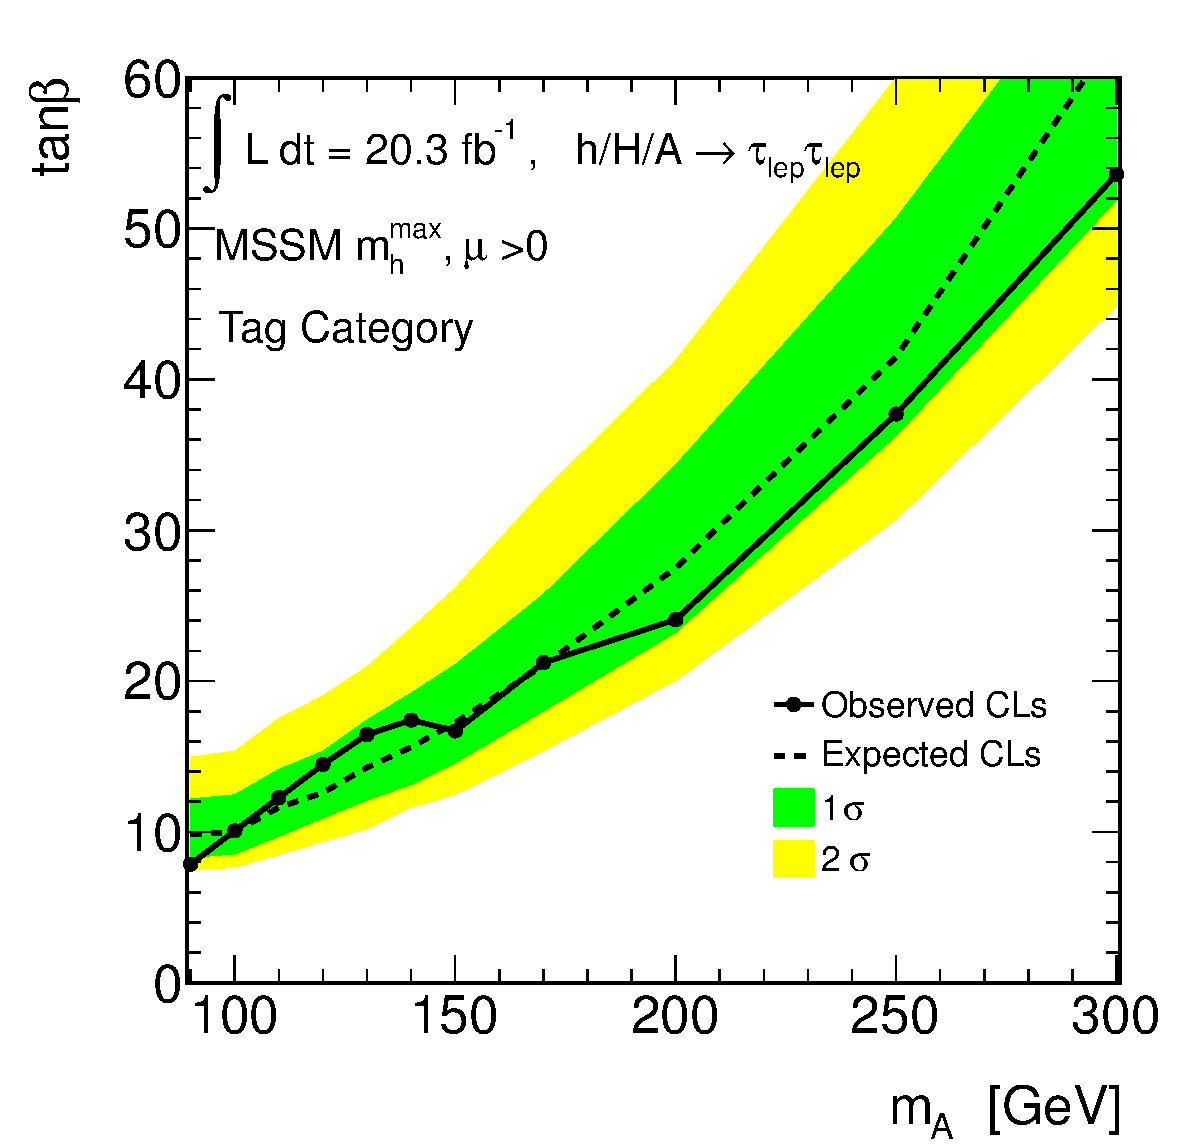
\includegraphics[width=0.6\textwidth]{figure/limits/tag_final.pdf}
  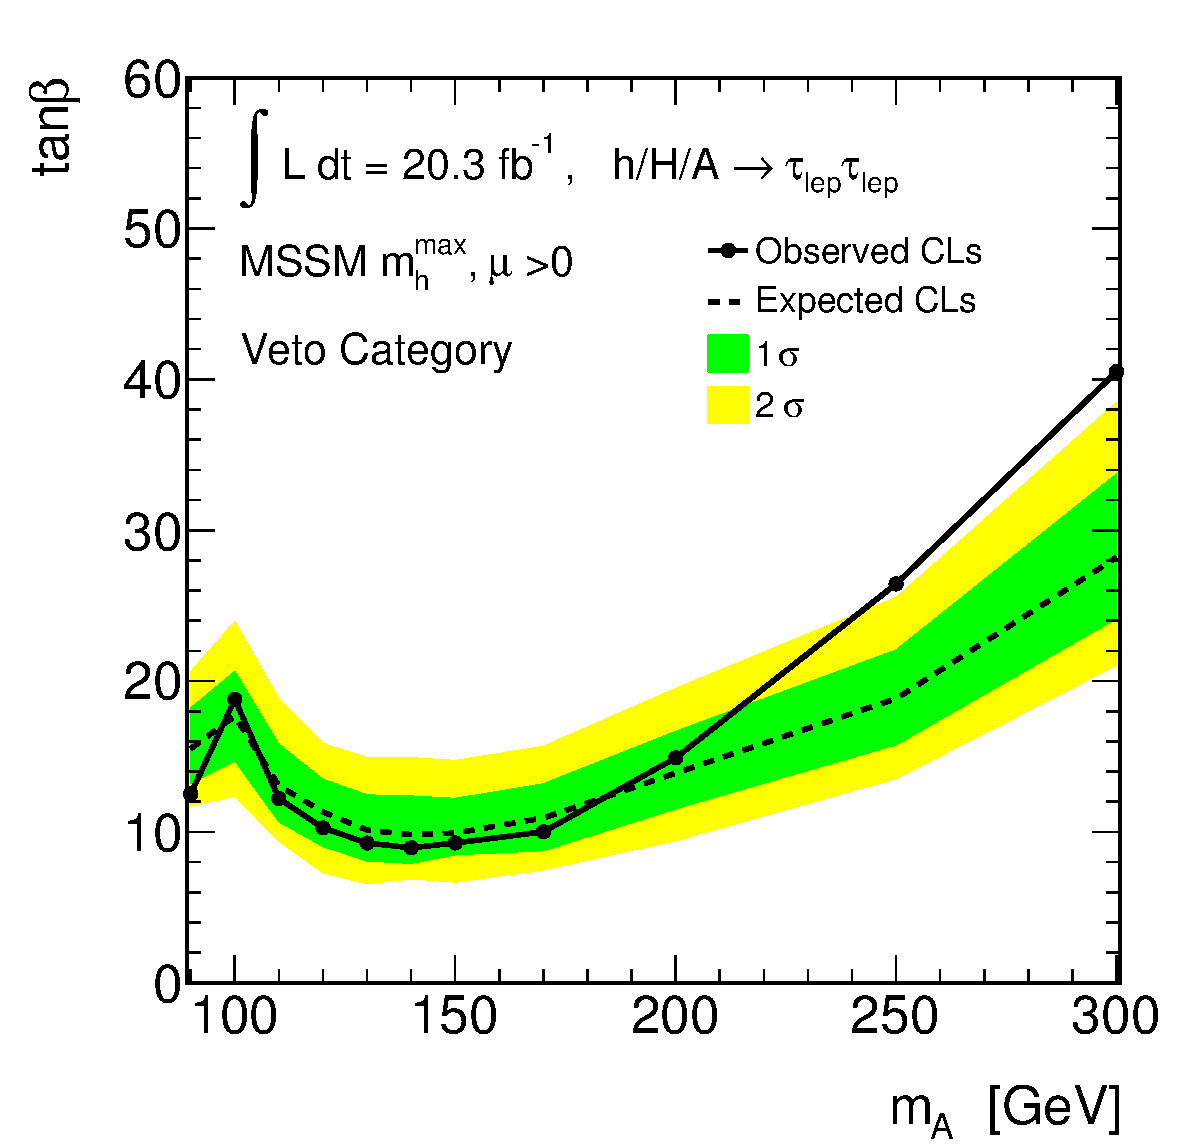
\includegraphics[width=0.6\textwidth]{figure/limits/veto_reg_spin.pdf}
  \caption{Expected and observed  exclusion limits at the $95\%$ $CL_s$ confidence-level for MSSM Higgs bosons production 
   interpreted in the  $m_A - \tan\beta$ parameter space of the $m_h^{max}$ scenario in the   b-tagged (top) and b-vetoed (bottom) category.}
\label{fig:limit_extract_combined2}
\end{figure}


\begin{figure}[!h]
     \begin{center}
	
            \includegraphics[page=3, width=0.47\textwidth]{figure/final_plots/Bveto_final.pdf}
            \includegraphics[page=4, width=0.47\textwidth]{figure/final_plots/Bveto_final.pdf}
            \includegraphics[page=6, width=0.47\textwidth]{figure/final_plots/Bveto_final.pdf}
            \includegraphics[page=9, width=0.47\textwidth]{figure/final_plots/Bveto_final.pdf}
    \end{center}
    \caption{ Observed and expected distribution for different kinematical variables after full selection of the b-tagged category.
	 In the ratio, the yellow and red band represents the systematic and statistical uncertainty in the background model prediction, 
	respectively,  while the error bars respresent the statistical uncertainty of data.}
\end{figure}

\begin{figure}[!p]
     \begin{center}
	
            \includegraphics[page=9, width=0.47\textwidth]{figure/final_plots/BTag_fulll.pdf}
            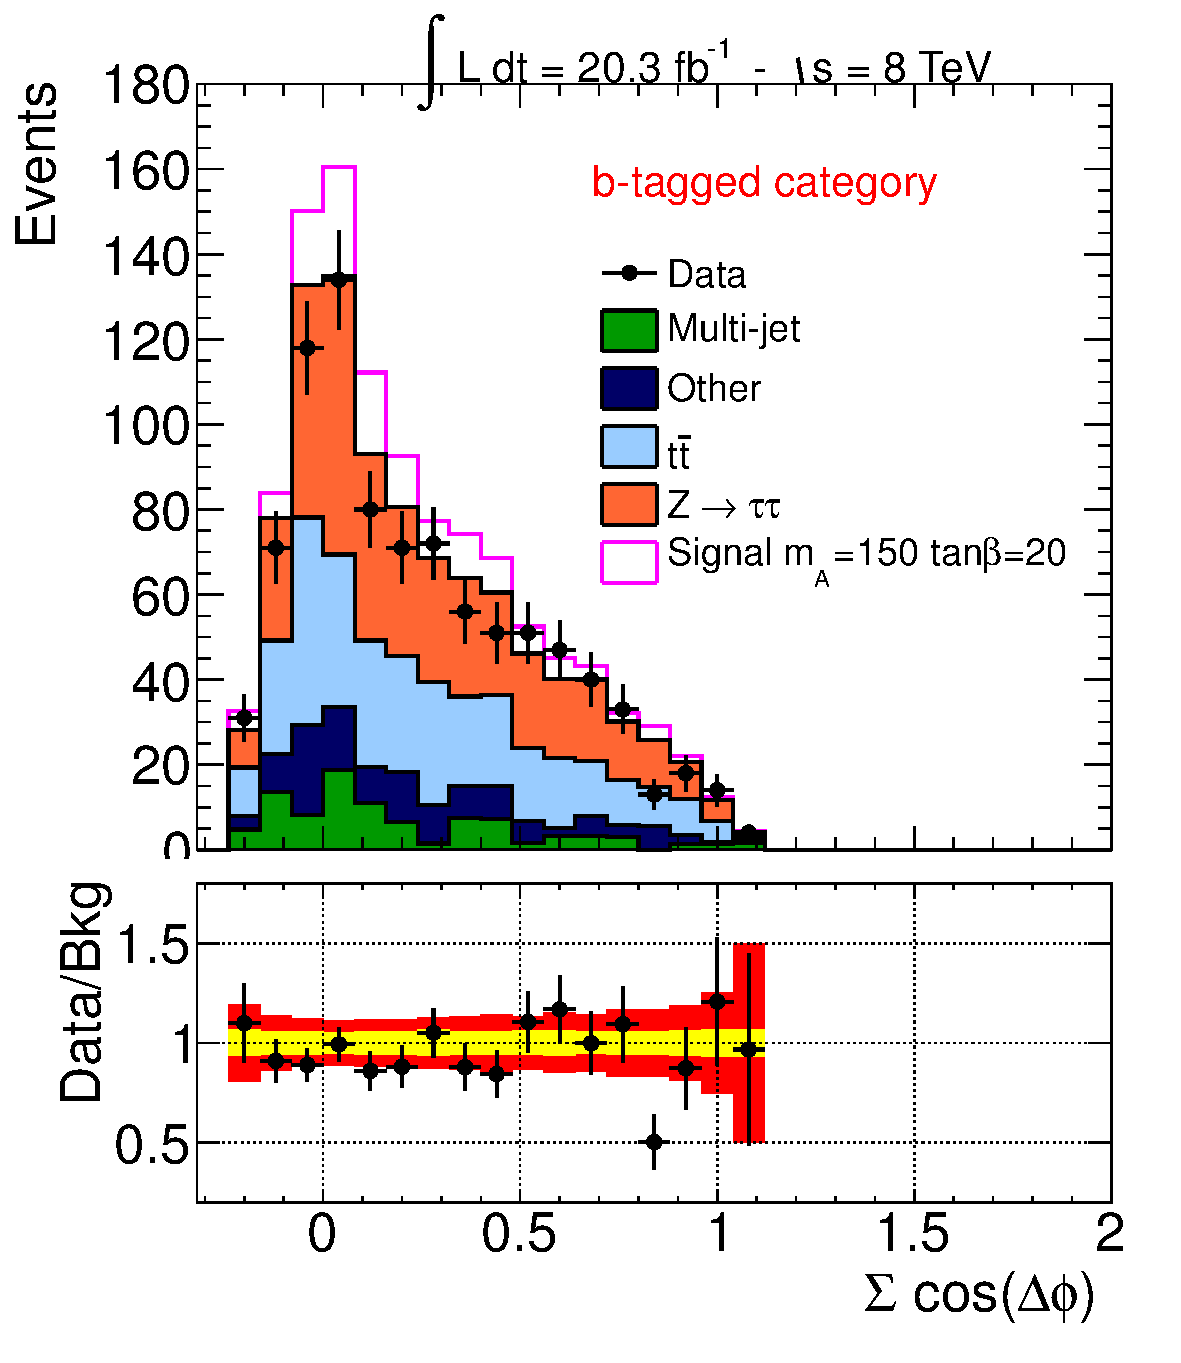
\includegraphics[page=1, width=0.47\textwidth]{figure/final_plots/BTag_fulll.pdf}
            \includegraphics[page=2, width=0.47\textwidth]{figure/final_plots/BTag_fulll.pdf}
            \includegraphics[page=6, width=0.47\textwidth]{figure/final_plots/BTag_fulll.pdf}
    \end{center}
    \caption{ Observed and expected distribution fori different kinematical variables after full selection of the b-tagged category.
	 In the ratio, the yellow and red band represents the systematic and statistical uncertainty in the background model prediction, 
	respectively,  while the error bars respresent the statistical uncertainty of data.}
\end{figure}


\clearpage

\chapter{Further Details on Limit}
\label{appendix:limit}

\section{The ABCD Method }
%How ABCD  is actually implemented in limits machinery
The actual implementation in the limit framework of the ABCD method follows that suggested in~\cite{ABCD}.
The control data samples B,C and D are considered as additional channels to be statistically combined
to two the signal event category. Three free parameters are fitted in B,C and D channels which are: the 
number of multi-jet events in the data sample B, $N_{B}^{QCD}$, the factor \rqcd 
and the factor that extrapolates from isolated to anti-isolated data control samples $R_{BD}$. Neglecting signal contributions, 
the following equations can be written for the event yield of the B,C and D control data samples:
%$$N_{B} = N_{B}^{BKG} + N_{B}^{QCD} $$ 
%$$N_{C} = N_{C}^{BKG} +  N_{B}^{QCD} \times \rqcd \times R_{BD} $$
%$$N_{D} =  N_{D}^{BKG} + N_{B}^{QCD} \times  R_{BD} $$
\begin{itemize}
\item[] $N_{B} = N_{B}^{BKG} + N_{B}^{QCD}$
\item[] $N_{C} = N_{C}^{BKG} +  N_{B}^{QCD} \times \rqcd \times R_{BD} $
\item[] $N_{D} =  N_{D}^{BKG} + N_{B}^{QCD} \times  R_{BD} $
\end{itemize}
where $N^{BKG}$ represent the prediction of  non-QCD background in the relative data samples.
The estimate of multi-jet event yield in the signal sample will be then $ N_{B}^{QCD} \times \rqcd $. This method is 
particularly powerful because in the best fit of \rqcd the statistical 
and systematics uncertainty for non-QCD backgrounds and data are considered.

\clearpage

\section{Shape Systematics} \label{appendix:shapeNPs}

\begin{figure}[!h]
     \begin{center}
	\subfigure[]{	
            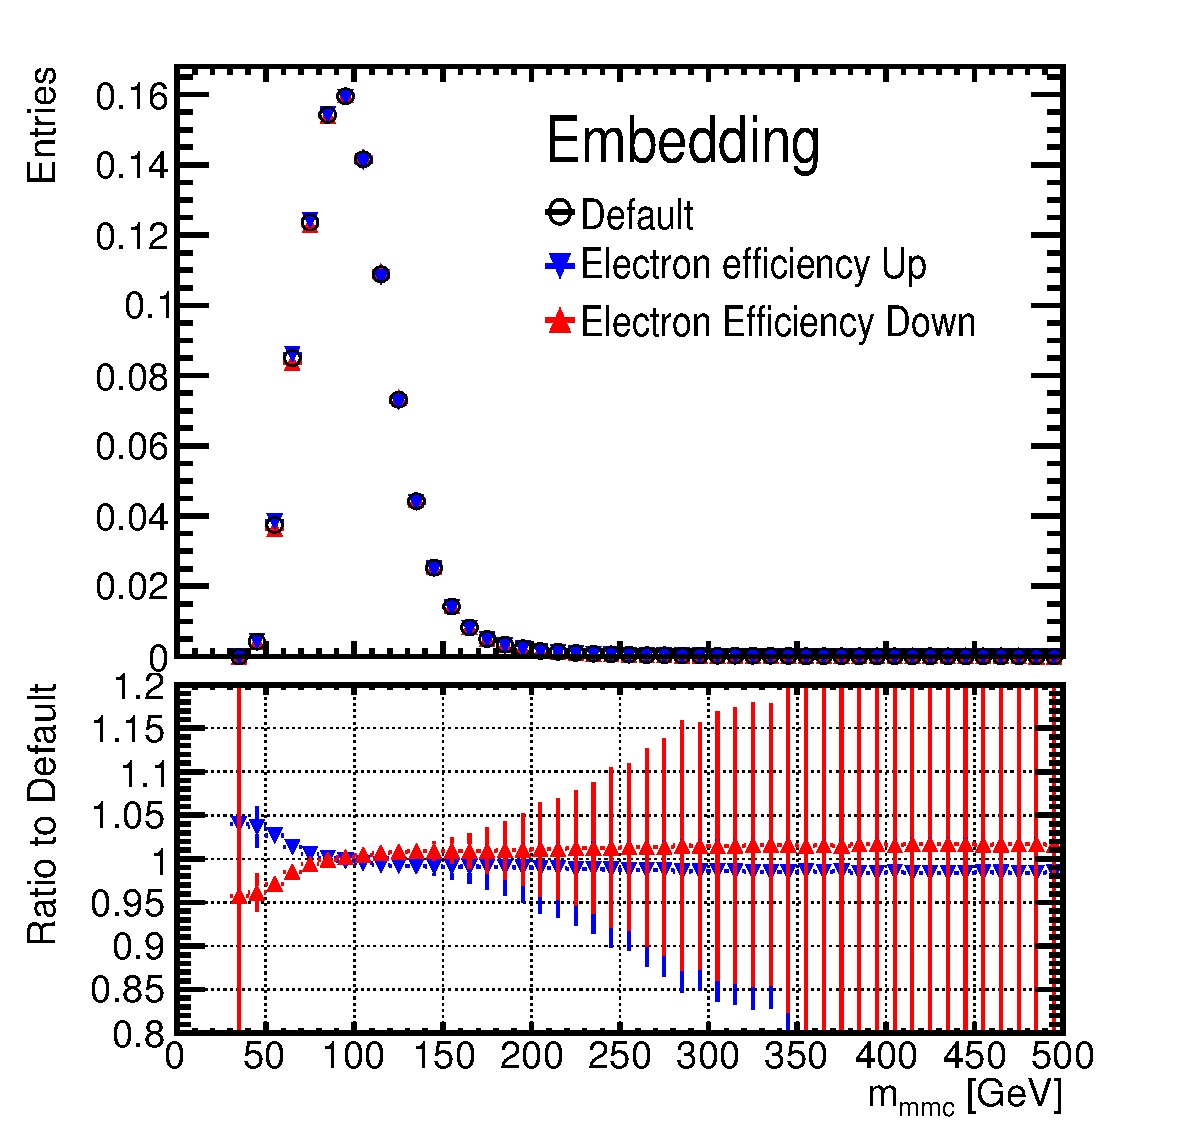
\includegraphics[width=0.47\textwidth]{figure/distributions/NP_Shape_ElecSF_BVeto_mmc.pdf}
	}
	\subfigure[]{	
            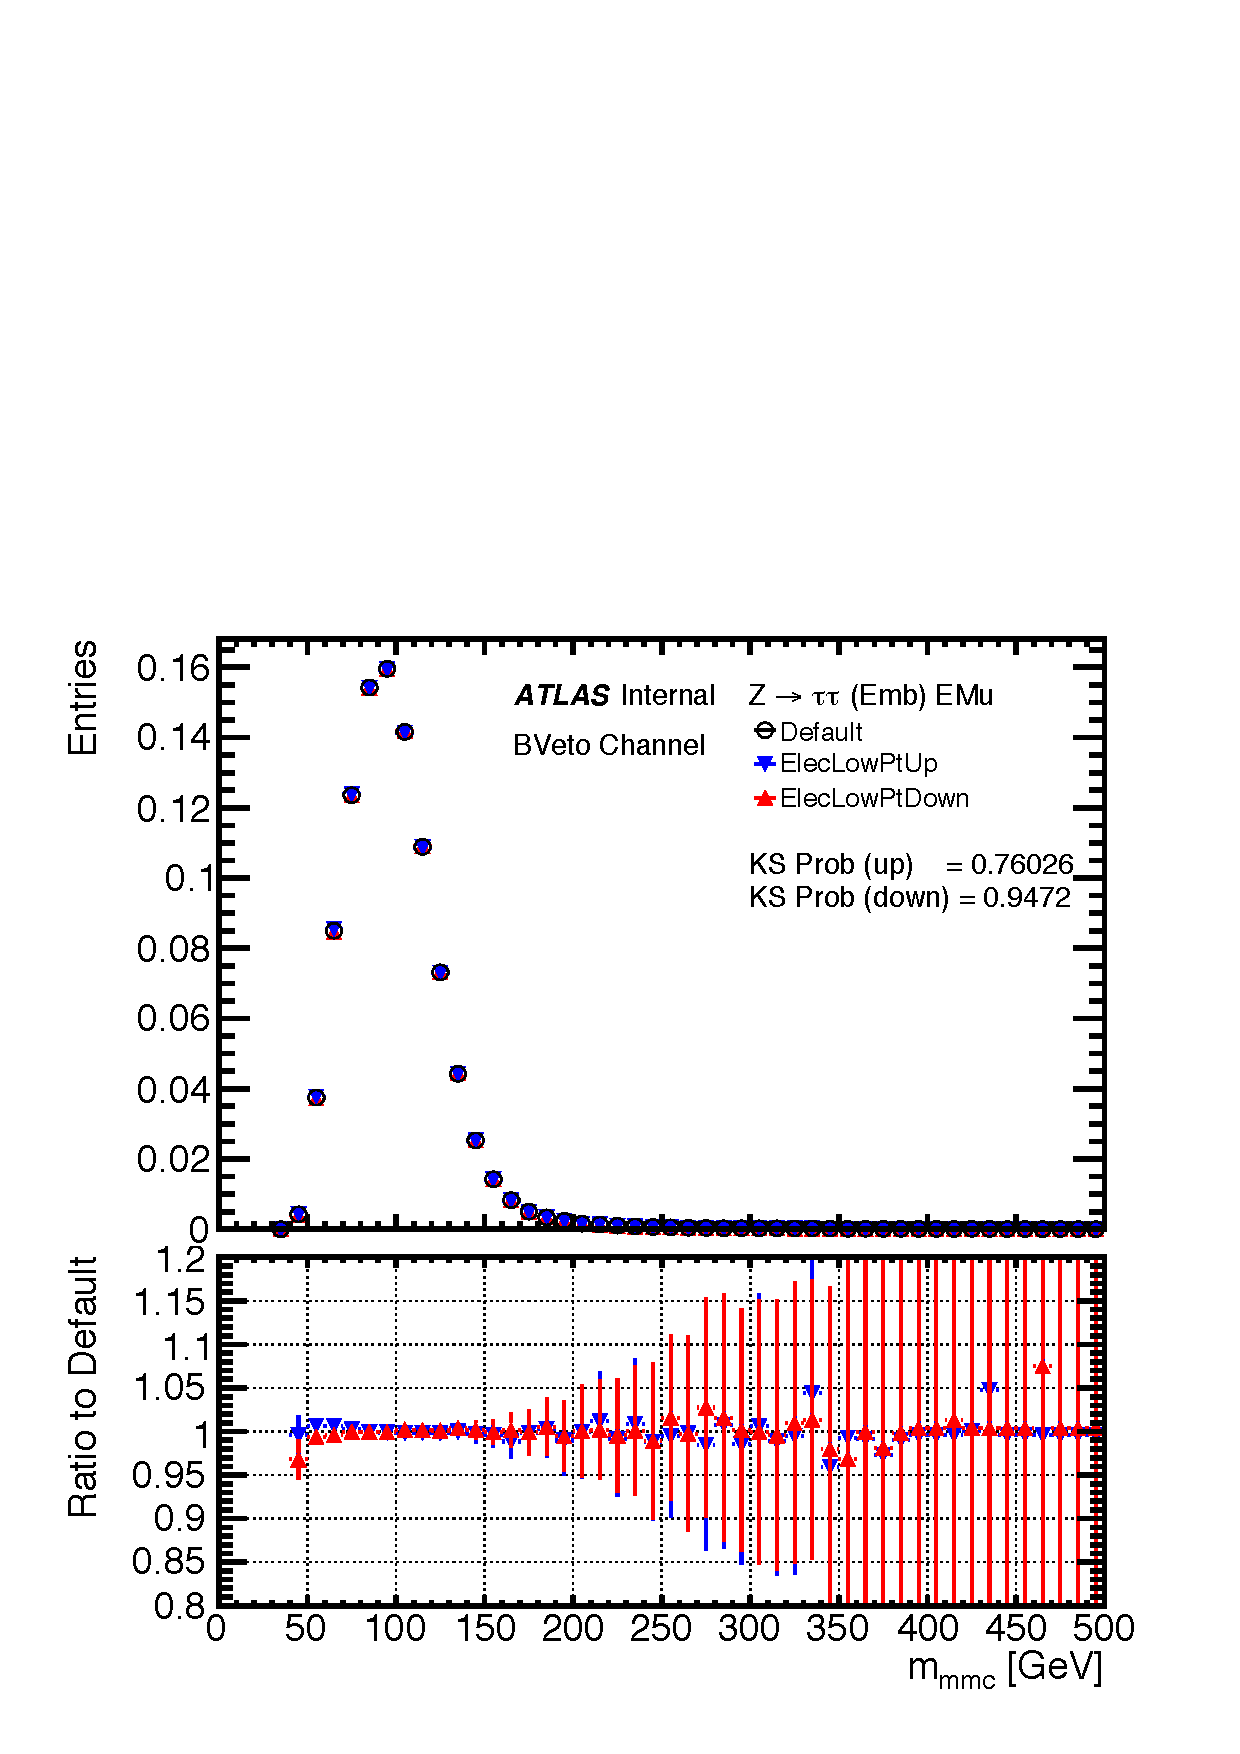
\includegraphics[width=0.47\textwidth]{figure/distributions/NP_Shape_ElecLowPt_BVeto_mmc.pdf}
	}
	\subfigure[]{	
            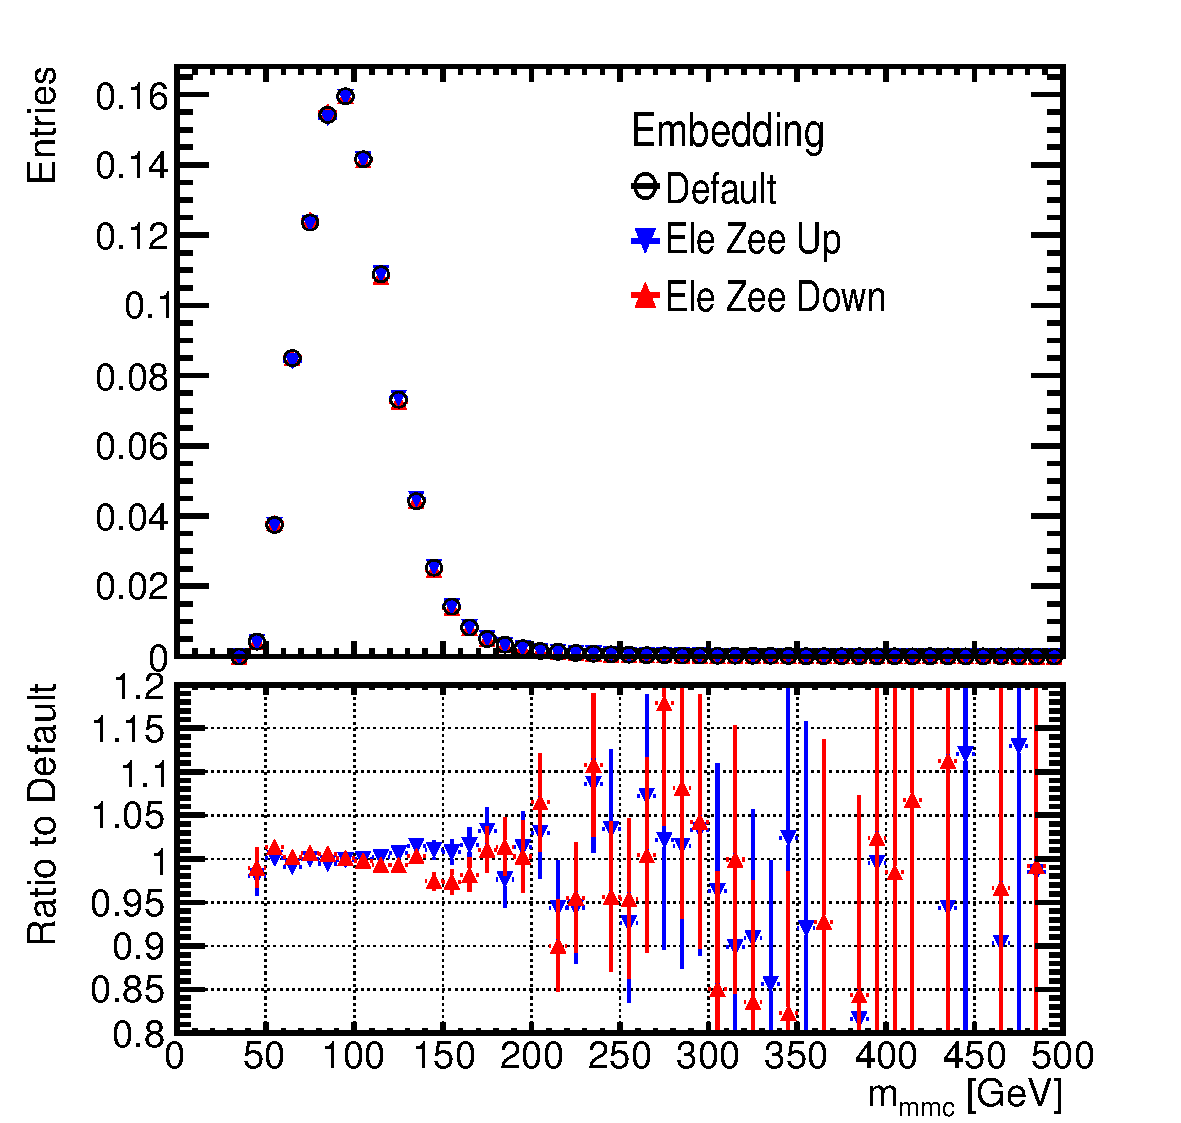
\includegraphics[width=0.47\textwidth]{figure/distributions/NP_Shape_ElecZee_BVeto_mmc.pdf}
	}
    \end{center}
    \caption{Effect on the \mmc distribution of the embedding sample due to the (a) the electron reconstruction and identification systematics, (b) the electron low \pt~ energy scale systematic and (c) the electron Zee energy scale systematic. The plots are made after the full b-veto category selection. Plots 
	provided by Matthew Backingham.}
\end{figure}

\clearpage

\section{Additional Limit Checks}
During the limit derivation, the systematic uncertainties (translated in term of nuisance parameter) are fitted to the data,
several checks are have been performed to ensure the quality of our statistical model.
If some of the nuisance parameters are significantly different from their nominal value 
(ie before fit), it can be symptomatic of an important mis-modelling and must be carefully scrutinised.
Also the correlation between the nuisance parameter and the signal strength (which reflects the degeneracy of the fit) 
is an important element to keep under control, in fact it reflects how well the data can constraint the nuisance parameters.
Finally, to have a feeling of the behaviour of the likelihood at its minimum one can check 
the negative log likelihood profile in each nuisance parameter direction. 
We performed all this checks using the package NuisanceCheck-00-00-05 described in \cite{NPcheck}.

The signal and background model with the signal normalisation free (unconditional fit) is fitted to the data,
in the following example plots the signal is assumed for the mass point mA~=~120 GeV, tan$\beta$~=~20,  
The difference between the post fit and pre-fit value of the nuisance parameter along with their errors is shown in Figure~\ref{fig:np_pull_comb}
for the combination between the two categories.
Figure~\ref{fig:np_correlation_comb} shows the correlation matrix between the nuisance parameters for the combination between the two channels.
Figure~\ref{fig:llh_1}-\ref{fig:llh_3} shows the behaviour of the likelihood at its minimum for 
each of the nuisance parameters (while a nuisance parameter is investigated the other are kept constant) for the combination between the channels.
%%%%%%%%%%%%%%%%%%%%%%%%%%%%%%%%%%%%%%%%%%%%%%% PULLS %%%%%%%%%%%%%%%%%%%%%%%%%%%%%%%%%%%%%%%%%%%%%%%%%%%%%%%%%%

\begin{figure}[htp]
     \begin{center}

            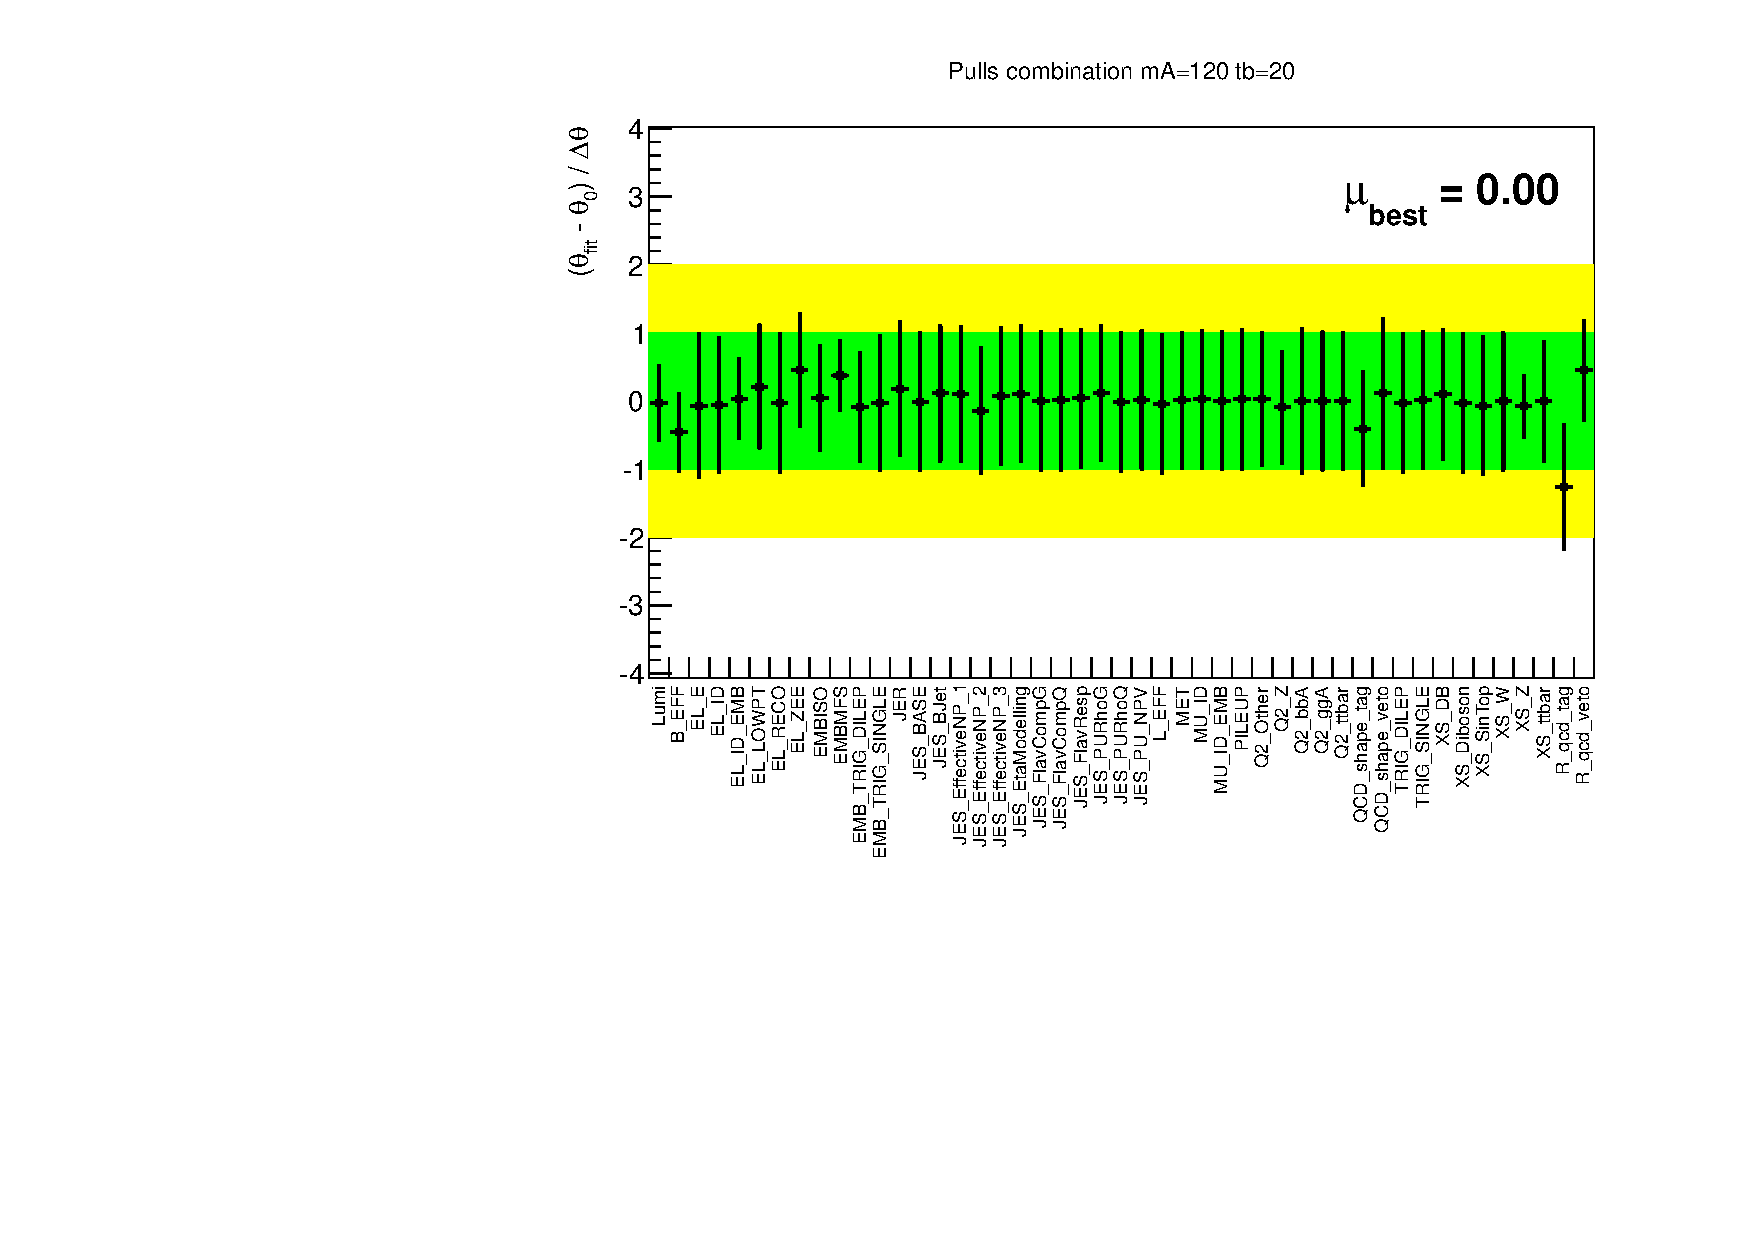
\includegraphics[width=\textwidth]{figure/np_check/120_comb_pulls.pdf}
            %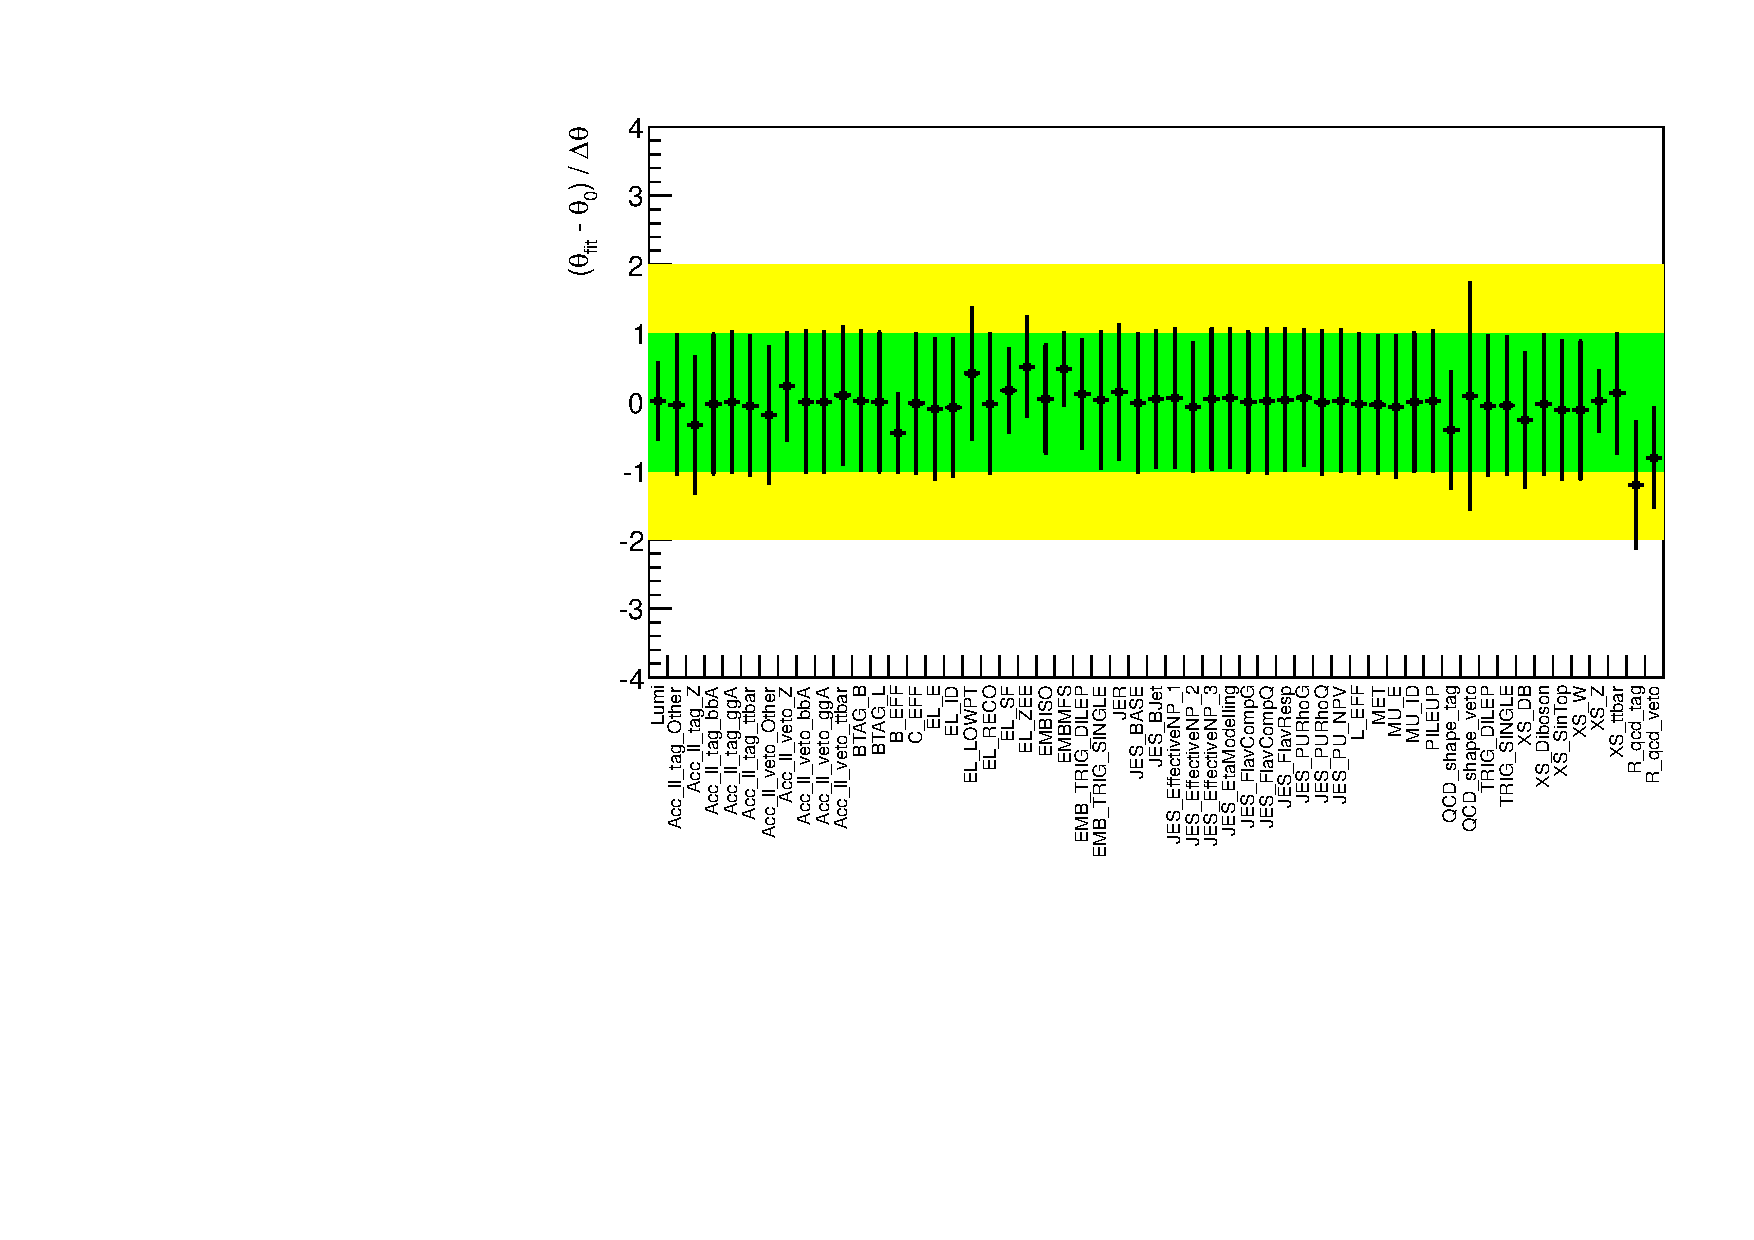
\includegraphics[width=\textwidth]{figure/np_check/pulls_combined.pdf}
    \end{center}
    \caption{ Pulls for nuisance parameter considered in the fit,  mA = 120 GeV, tan$\beta$ = 20, combination between the two channel. These pulls are obtained with
	NuissanceCheck package, using asymptotic approximation.} 
    \label{fig:np_pull_comb}
\end{figure}
%%%%%%%%%%%%%%%%%%%%%%%%%%%%%%%%%%%%%%%%%%%%%%%  %%%%%%%%%%%%%%%%%%%%%%%%%%%%%%%%%%%%%%%%%%%%%%%%%%%%%%%%%%

%%%%%%%%%%%%%%%%%%%%%%%%%%%%%%%%%%%%%%%%%%%%%%% CORRELATION MATRIX %%%%%%%%%%%%%%%%%%%%%%%%%%%%%%%%%%%%%%%%%%%%%%%%%%%%%%%%%%
\begin{figure}[htp]
     \begin{center}

           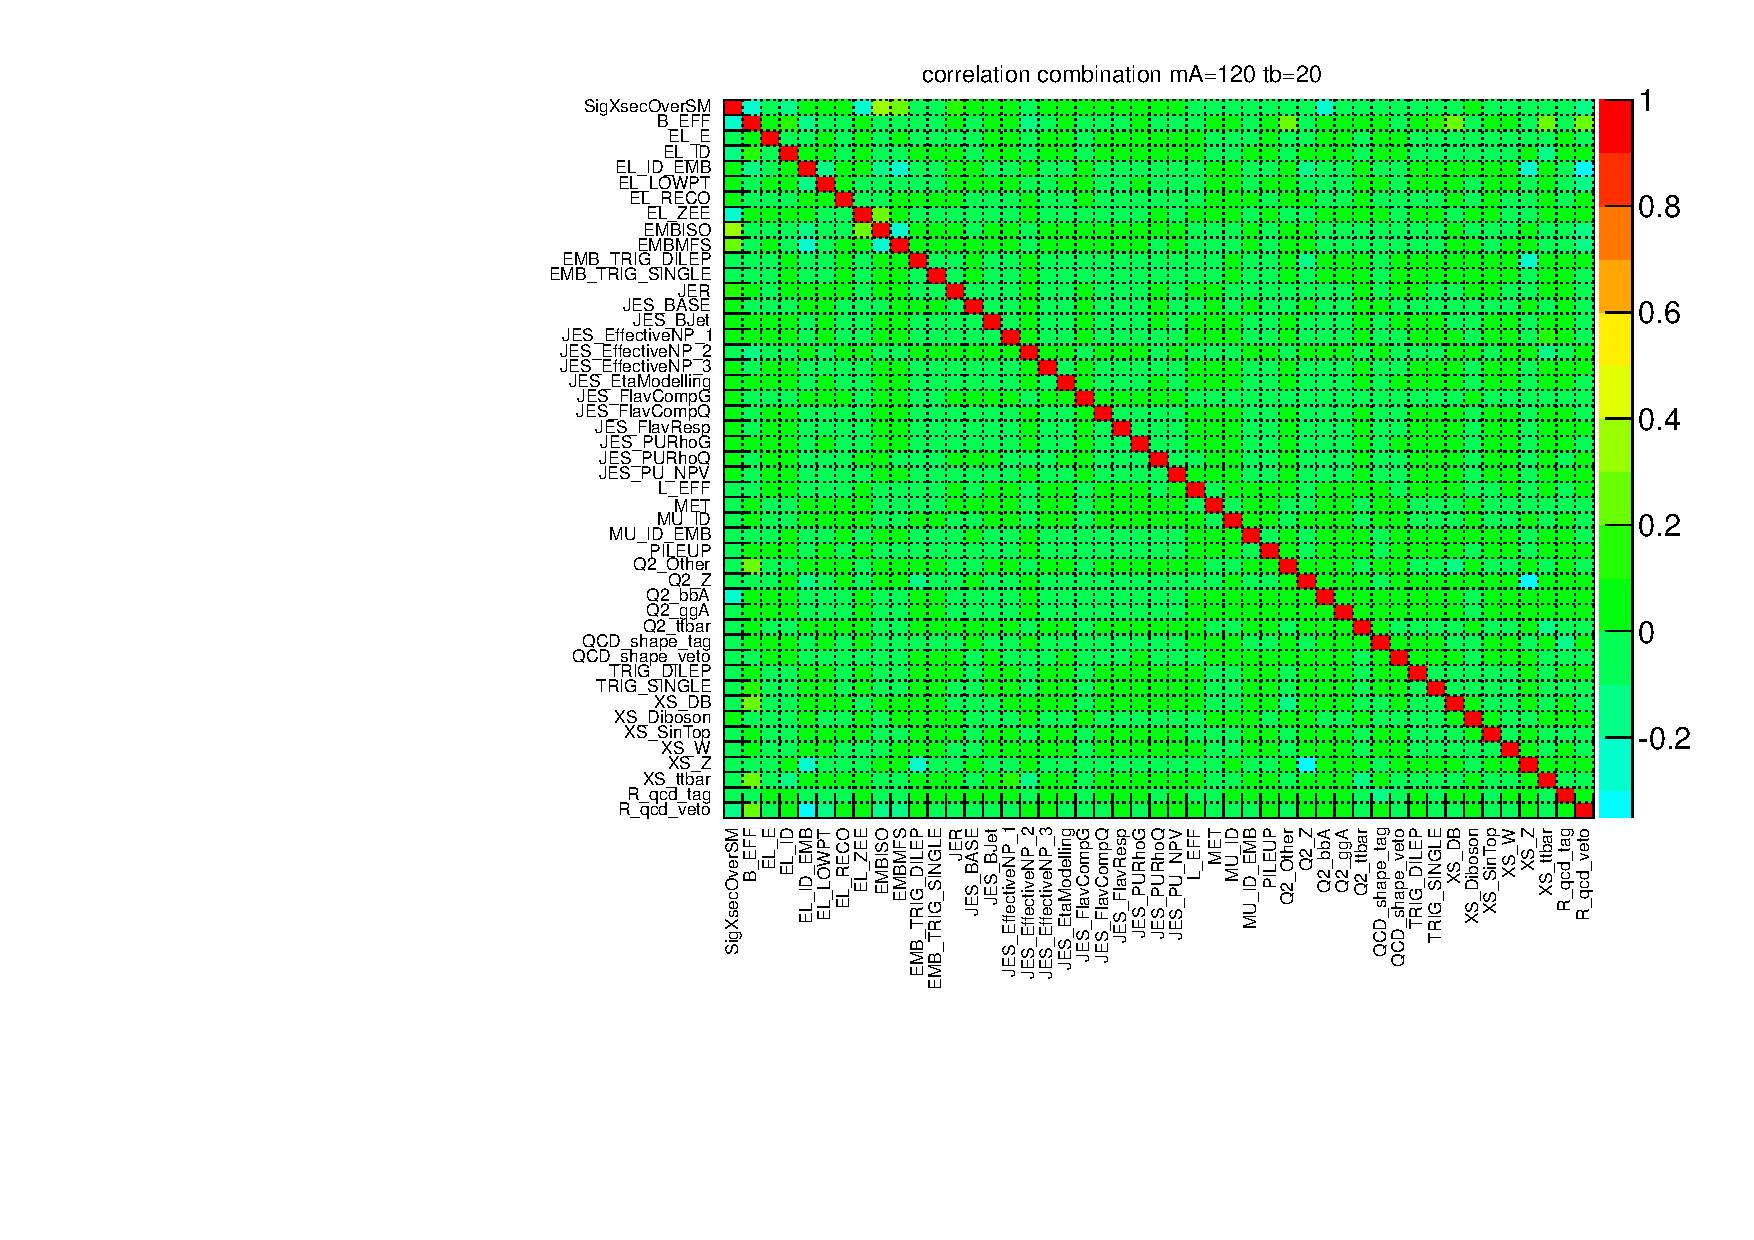
\includegraphics[width=1.1\textwidth]{figure/np_check/matrix_comb_120.pdf}
           %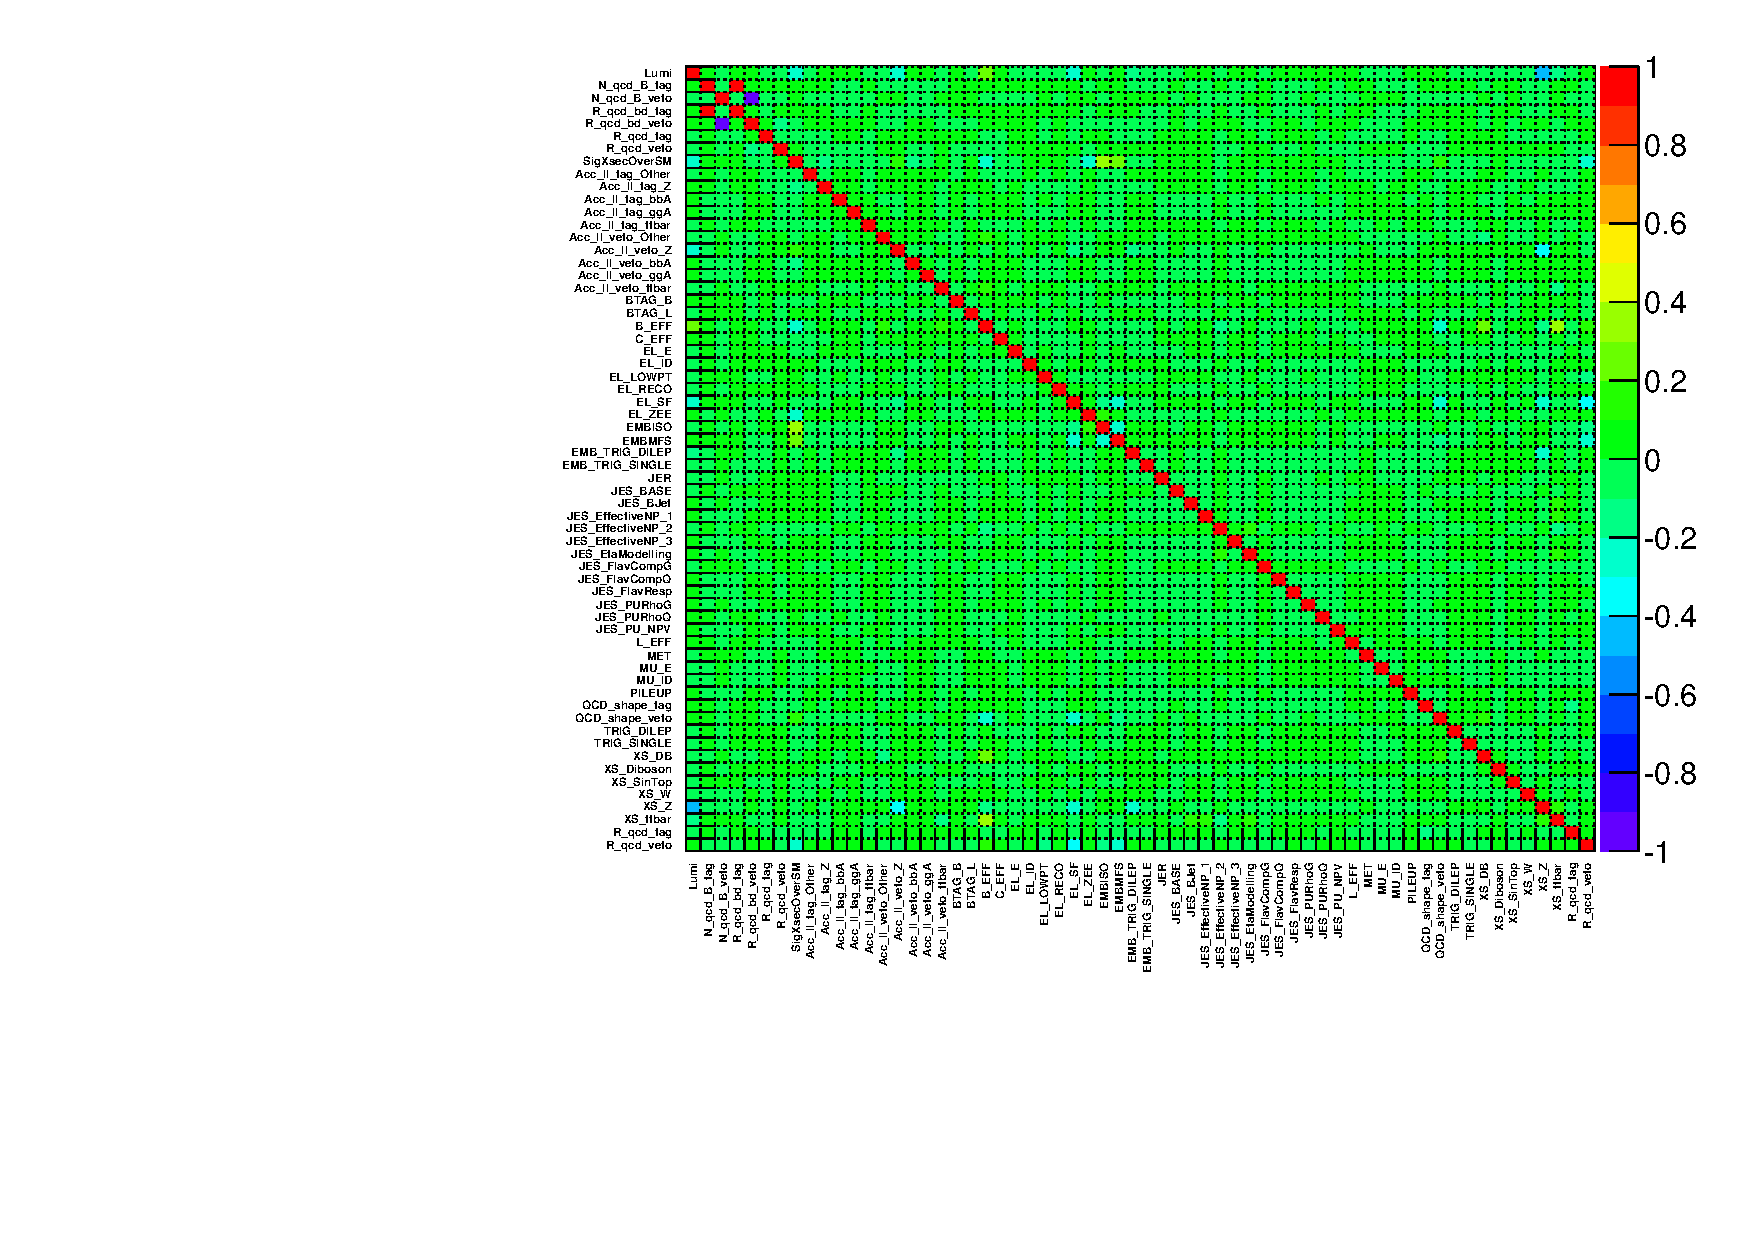
\includegraphics[width=1.1\textwidth]{figure/np_check/matrix_combined.pdf}
    \end{center}
    \caption{ Correlation matrix for nuisance parameters considered in the fit.  The point mA = 120 GeV and tan$\beta$ = 20 is 
	considered for the combination of the b-tag and b-veto channels. This correlation matrix is obtained with 
	NuissanceCheck package, using asymptotic approximation.} 
    \label{fig:np_correlation_comb}
\end{figure}
%%%%%%%%%%%%%%%%%%%%%%%%%%%%%%%%%%%%%%%%%%%%%%%  %%%%%%%%%%%%%%%%%%%%%%%%%%%%%%%%%%%%%%%%%%%%%%%%%%%%%%%%%%

%%%%%%%%%%%%%%%%%%%%%%%%%%%%%%%%%%%%%%%%%%%%%%% llh SCANS %%%%%%%%%%%%%%%%%%%%%%%%%%%%%%%%%%%%%%%%%%%%%%%%%%%%%%%%%%

\begin{figure}[htp]
     \begin{center}

            \includegraphics[page=8,width=0.3\textwidth]{figure/np_check/comb_LLHscan_f.pdf}
            \includegraphics[page=9,width=0.3\textwidth]{figure/np_check/comb_LLHscan_f.pdf}
            \includegraphics[page=10,width=0.3\textwidth]{figure/np_check/comb_LLHscan_f.pdf}\\
            \includegraphics[page=11,width=0.3\textwidth]{figure/np_check/comb_LLHscan_f.pdf}
            \includegraphics[page=12,width=0.3\textwidth]{figure/np_check/comb_LLHscan_f.pdf}
            \includegraphics[page=13,width=0.3\textwidth]{figure/np_check/comb_LLHscan_f.pdf}\\
            \includegraphics[page=14,width=0.3\textwidth]{figure/np_check/comb_LLHscan_f.pdf}
            \includegraphics[page=15,width=0.3\textwidth]{figure/np_check/comb_LLHscan_f.pdf}
            \includegraphics[page=16,width=0.3\textwidth]{figure/np_check/comb_LLHscan_f.pdf}\\
            \includegraphics[page=17,width=0.3\textwidth]{figure/np_check/comb_LLHscan_f.pdf}
            \includegraphics[page=18,width=0.3\textwidth]{figure/np_check/comb_LLHscan_f.pdf}
            \includegraphics[page=19,width=0.3\textwidth]{figure/np_check/comb_LLHscan_f.pdf}\\
            \includegraphics[page=20,width=0.3\textwidth]{figure/np_check/comb_LLHscan_f.pdf}
            \includegraphics[page=21,width=0.3\textwidth]{figure/np_check/comb_LLHscan_f.pdf}
            \includegraphics[page=22,width=0.3\textwidth]{figure/np_check/comb_LLHscan_f.pdf}\\

    \end{center}
    \caption{ Likelihood scans for nuisance parameter considered in the fit, mA = 120 GeV, tan$\beta$ = 20, combination between the two channel.} 
    \label{fig:llh_1}
\end{figure}

\begin{figure}[htp]
     \begin{center}

            \includegraphics[page=23,width=0.3\textwidth]{figure/np_check/comb_LLHscan_f.pdf}
            \includegraphics[page=24,width=0.3\textwidth]{figure/np_check/comb_LLHscan_f.pdf}
            \includegraphics[page=25,width=0.3\textwidth]{figure/np_check/comb_LLHscan_f.pdf}\\
            \includegraphics[page=26,width=0.3\textwidth]{figure/np_check/comb_LLHscan_f.pdf}
            \includegraphics[page=27,width=0.3\textwidth]{figure/np_check/comb_LLHscan_f.pdf}
            \includegraphics[page=28,width=0.3\textwidth]{figure/np_check/comb_LLHscan_f.pdf}\\
            \includegraphics[page=29,width=0.3\textwidth]{figure/np_check/comb_LLHscan_f.pdf}
            \includegraphics[page=30,width=0.3\textwidth]{figure/np_check/comb_LLHscan_f.pdf}
            \includegraphics[page=31,width=0.3\textwidth]{figure/np_check/comb_LLHscan_f.pdf}\\
            \includegraphics[page=32,width=0.3\textwidth]{figure/np_check/comb_LLHscan_f.pdf}
            \includegraphics[page=33,width=0.3\textwidth]{figure/np_check/comb_LLHscan_f.pdf}
            \includegraphics[page=34,width=0.3\textwidth]{figure/np_check/comb_LLHscan_f.pdf}\\
            \includegraphics[page=35,width=0.3\textwidth]{figure/np_check/comb_LLHscan_f.pdf}
            \includegraphics[page=36,width=0.3\textwidth]{figure/np_check/comb_LLHscan_f.pdf}
            \includegraphics[page=37,width=0.3\textwidth]{figure/np_check/comb_LLHscan_f.pdf}\\

    \end{center}
    \caption{ Likelihood scans for nuisance parameter considered in the fit,  mA = 120 GeV, tan$\beta$ = 20, combination between the two channel.} 
    \label{fig:llh_2}
\end{figure}


\begin{figure}[htp]
     \begin{center}

            \includegraphics[page=38,width=0.3\textwidth]{figure/np_check/comb_LLHscan_f.pdf}
            \includegraphics[page=39,width=0.3\textwidth]{figure/np_check/comb_LLHscan_f.pdf}
            \includegraphics[page=40,width=0.3\textwidth]{figure/np_check/comb_LLHscan_f.pdf}\\
            \includegraphics[page=41,width=0.3\textwidth]{figure/np_check/comb_LLHscan_f.pdf}
            \includegraphics[page=42,width=0.3\textwidth]{figure/np_check/comb_LLHscan_f.pdf}
            \includegraphics[page=43,width=0.3\textwidth]{figure/np_check/comb_LLHscan_f.pdf}\\
            \includegraphics[page=44,width=0.3\textwidth]{figure/np_check/comb_LLHscan_f.pdf}
            \includegraphics[page=45,width=0.3\textwidth]{figure/np_check/comb_LLHscan_f.pdf}
            \includegraphics[page=46,width=0.3\textwidth]{figure/np_check/comb_LLHscan_f.pdf}\\
            \includegraphics[page=47,width=0.3\textwidth]{figure/np_check/comb_LLHscan_f.pdf}
            \includegraphics[page=48,width=0.3\textwidth]{figure/np_check/comb_LLHscan_f.pdf}
            \includegraphics[page=49,width=0.3\textwidth]{figure/np_check/comb_LLHscan_f.pdf}\\
            \includegraphics[page=50,width=0.3\textwidth]{figure/np_check/comb_LLHscan_f.pdf}
            \includegraphics[page=51,width=0.3\textwidth]{figure/np_check/comb_LLHscan_f.pdf}
            \includegraphics[page=52,width=0.3\textwidth]{figure/np_check/comb_LLHscan_f.pdf}\\

    \end{center}
    \caption{ Likelihood scans for nuisance parameter considered in the fit,  mA = 120 GeV, tan$\beta$ = 20, combination between the two channel.} 
    \label{fig:llh_3}
\end{figure}

\clearpage
\subsection{Regularization of Signal Samples}

In the b-tag channel of this analysis, it is observed that the MC prediction of the signal yield has a relatively large statistical uncertainty. This, in turn, 
leads to statistical fluctuations on the expected limits derived from the b-tag channel. To counteract this effect, the signal yield at each mass 
point is rescaled using a fourth order polynomial fitted to the uncorrected signal yields as a function of the mass $\mathrm{m_A}$. The rescaled yeilds ar then used for both the cross section independent limits and those interpreted within the MSSM. Figure~\ref{fig:regularizzation} shows 
the uncorrected event yields as a function of $\mathrm{m_A}$, normalised using a cross section of 1~pb.  The red line shows the result of the fourth order polynomial fit 
to the signal yields. While the fit to the b-associated production signal yield leads to a smoothly varying function, the fit to the gluon fusion production 
yields is less so. However, since events from this production mode only have a small contribution to the total expected signal in the b-tag channel, the shape of this correction as a function of mA does not affect the final limits.


%In the b-tag category the signal histograms have a relatively large statistical uncertainty on their total yield,
%statistical fluctuation in the signal acceptance for different mass points has a sirius impact on the 
%expected limits. There is no reason to belive that two signal samples for the same production process
%and with very close mass should have drastically different acceptances. We rescale a signal sample representing a
% given mass point with the value obtained via a fit with a 4th grade
%polinom of the signal acceptance as a function of the mass points, this method reduces considerably 
%statistical fluctiation. In Figure~\ref{fig:regularizzation} the event yield for different mass point is fitted
%with a 4th grade polinom, the yield of each sample is evaluated considering for each of them a cross section of one pb.

\begin{figure}[!hb]
  \centering
  \includegraphics[width=0.47\textwidth]{figure/limits/bbA_regularizzation.pdf}
  \includegraphics[width=0.47\textwidth]{figure/limits/ggH_regularizzation.pdf}
  \caption{Fit of the uncorrected event yield for different mass points for the signal produced via b-associate production (top)
and gluon-fusion (bottom) for the b-tag category. Each mass point is normalised using a signal cross section of 1~pb.}
\label{fig:regularizzation}
\end{figure}

\clearpage
\subsection{Pre Fit and Post Fit MMC mass Plots}

\begin{figure}[!hb]
  \centering
  \includegraphics[width=0.6\textwidth]{figure/limits/post_fit_250.pdf}
  \includegraphics[width=0.6\textwidth]{figure/limits/post_fit_ma300.pdf}
  \caption{Post-fit \mmc mass distribution for the veto category final selections. A signal is injected with 
	$m_A=250$ (top) and  $m_A=300$ (bottom) for $\tan\beta=20$ assuming $m_h^{max}$ scenario. The 1$\sigma$ bands 
	represent the statistical and systematic uncertainties.  }

\end{figure}

\begin{figure}[!hb]
  \centering
  \includegraphics[width=0.7\textwidth]{figure/limits/pulls_250.pdf}
  \caption{Pulls for unconditional fit for the b-veto category. A signal is injected with 
	$m_A=250$ and  $\tan\beta=20$ assuming $m_h^{max}$ scenario. The pulls are obtained with NuissanceCheck package.  }

\end{figure}

\begin{figure}[!hb]
  \centering
  \includegraphics[width=0.7\textwidth]{figure/limits/matrix_250.pdf}
  \caption{Correlation matrix for unconditional fit for the b-veto category. A signal is injected with 
	$m_A=250$ and  $\tan\beta=20$ assuming $m_h^{max}$ scenario. The pulls are obtained with NuissanceCheck package.  }

\end{figure}

\begin{figure}[!hb]
  \centering
  \includegraphics[width=0.7\textwidth]{figure/limits/pulls_300.pdf}
  \caption{Pulls for unconditional fit for the b-veto category. A signal is injected with 
	$m_A=300$ and  $\tan\beta=20$ assuming $m_h^{max}$ scenario. The pulls are obtained with NuissanceCheck package.  }

\end{figure}

\begin{figure}[!hb]
  \centering
  \includegraphics[width=0.7\textwidth]{figure/limits/matrix_300.pdf}
  \caption{Correlation matrix for unconditional fit for the b-veto category. A signal is injected with 
	$m_A=300$ and  $\tan\beta=20$ assuming $m_h^{max}$ scenario. The pulls are obtained with NuissanceCheck package.  }

\end{figure}


\clearpage
\subsection{Checks in Mass range 230-300 GeV}
\begin{figure}[!hb]
  \centering
  \includegraphics[page=1,width=0.47\textwidth]{figure/limits/vetoM230_300.pdf}
  \includegraphics[page=2,width=0.47\textwidth]{figure/limits/vetoM230_300.pdf}
  \caption{Pre-fit distribution of \mmc mass for the veto category final selections. A mass vindow selection is applied 
	selecting only the mass range $230 < \mmc < 300 $~GeV. The case of muon or electron being the leading lepton are shown separately.
	A signal is injected assiuming gluon fusion production of a scalar boson $\phi$ with mass $m_{\phi} = 250$~GeV, its cross section
	is normalized to $2.4\times5~pb$. Since electron fakes are more likely than muon fakes, in case of $W$ boson mismodeling an
	excess is expected in the distribution of leading muon events.}

\end{figure}

\begin{figure}[!hb]
  \centering
  \includegraphics[page=3,width=0.47\textwidth]{figure/limits/vetoM230_300.pdf}
  \includegraphics[page=4,width=0.47\textwidth]{figure/limits/vetoM230_300.pdf}
  \includegraphics[page=5,width=0.47\textwidth]{figure/limits/vetoM230_300.pdf}
  \caption{Pre-fit distribution of different kinematic variables for the veto category final selections. A mass vindow selection is applied 
	selecting only the mass range $230 < \mmc < 300 $~GeV. 
	A signal is injected assiuming gluon fusion production of a scalar boson $\phi$ with mass $m_{\phi} = 250$~GeV, its cross section
	is normalized to $2.4\times5~pb$.}

\end{figure}
\clearpage
